\documentclass[11pt,a4paper]{article}

% ── Packages ──────────────────────────────────────────────────────────────────
\usepackage[top=2.8cm, bottom=2.8cm, left=3cm, right=3cm]{geometry}
\usepackage[T1]{fontenc}
\usepackage[utf8]{inputenc}
\usepackage{lmodern}
\usepackage{microtype}
\usepackage[colorlinks=true, linkcolor=linkblue, urlcolor=accent,
            pdftitle={L1-01 Networking -- System Design Foundations},
            bookmarks=true]{hyperref}
\usepackage{xcolor}
\usepackage{titlesec}
\usepackage{enumitem}
\usepackage{booktabs}
\usepackage{tabularx}
\usepackage{tcolorbox}
\usepackage{fancyhdr}
\usepackage{amsmath}
\usepackage{parskip}
\usepackage{mdframed}
\usepackage{graphicx}
\usepackage{tikz}
\usepackage{setspace}
\usepackage{soul}
\usepackage{marginnote}

% ── Colors ────────────────────────────────────────────────────────────────────
\definecolor{primary}{HTML}{1A1A2E}
\definecolor{accent}{HTML}{C0392B}
\definecolor{highlight}{HTML}{1A5276}
\definecolor{linkblue}{HTML}{154360}
\definecolor{lightbg}{HTML}{F4F6F7}
\definecolor{warnbg}{HTML}{FEF9E7}
\definecolor{quizbg}{HTML}{EBF5FB}
\definecolor{termbg}{HTML}{EAF2FF}
\definecolor{curiobg}{HTML}{F5EEF8}
\definecolor{greenbg}{HTML}{EAFAF1}
\definecolor{notebg}{HTML}{FDF2E9}
\definecolor{accentlight}{HTML}{FADBD8}

% ── Section styling ───────────────────────────────────────────────────────────
\titleformat{\section}
  {\large\bfseries\color{highlight}}
  {\thesection.}{0.6em}{}
  [\vspace{2pt}\color{highlight!60}\rule{\linewidth}{0.6pt}]

\titleformat{\subsection}
  {\normalsize\bfseries\color{primary}}
  {\thesubsection}{0.5em}{}

\titleformat{\subsubsection}
  {\normalsize\itshape\color{primary!80}}
  {}{0em}{}

\titlespacing{\section}{0pt}{18pt}{8pt}
\titlespacing{\subsection}{0pt}{12pt}{4pt}
\titlespacing{\subsubsection}{0pt}{8pt}{2pt}

% ── Header/Footer ─────────────────────────────────────────────────────────────
\pagestyle{fancy}
\fancyhf{}
\fancyhead[L]{\small\color{highlight}\textbf{L1-01 --- Networking Fundamentals}}
\fancyhead[R]{\small\color{primary!70}System Design Interview Prep}
\fancyfoot[C]{\small\color{primary!60}\thepage}
\renewcommand{\headrulewidth}{0.4pt}
\renewcommand{\headrule}{\hbox to\headwidth{\color{highlight!40}\leaders\hrule height \headrulewidth\hfill}}

% ── Box environments ──────────────────────────────────────────────────────────
\tcbuselibrary{skins, breakable, hooks}

% Concept definition box
\newtcolorbox{termbox}[1]{
  enhanced, breakable,
  colback=termbg,
  colframe=highlight,
  coltitle=white,
  fonttitle=\bfseries\small,
  title={#1},
  left=8pt, right=8pt, top=6pt, bottom=6pt,
  attach boxed title to top left={yshift=-2.5mm, xshift=6mm},
  boxed title style={colback=highlight, sharp corners, left=4pt, right=4pt}
}

% Industry data box
\newtcolorbox{industrybox}[1]{
  enhanced, breakable,
  colback=greenbg,
  colframe=highlight!50!black,
  coltitle=white,
  fonttitle=\bfseries\small,
  title={Industry Data: #1},
  left=8pt, right=8pt, top=6pt, bottom=6pt,
  attach boxed title to top left={yshift=-2.5mm, xshift=6mm},
  boxed title style={colback=highlight!60!black, sharp corners, left=4pt, right=4pt}
}

% Warning / trap box
\newtcolorbox{trapbox}[1]{
  enhanced,
  colback=accentlight,
  colframe=accent,
  coltitle=white,
  fonttitle=\bfseries\small,
  title={Interview Trap: #1},
  left=8pt, right=8pt, top=6pt, bottom=6pt,
  attach boxed title to top left={yshift=-2.5mm, xshift=6mm},
  boxed title style={colback=accent, sharp corners, left=4pt, right=4pt}
}

% Think-about-it box
\newtcolorbox{thinkbox}{
  enhanced,
  colback=notebg,
  colframe=accent!60,
  left=8pt, right=8pt, top=6pt, bottom=6pt,
  leftrule=3pt, rightrule=0pt, toprule=0pt, bottomrule=0pt,
}

% Curiosity corner answer
\newtcolorbox{curiobox}[1]{
  enhanced, breakable,
  colback=curiobg,
  colframe=primary!60,
  coltitle=white,
  fonttitle=\bfseries\small,
  title={Q: #1},
  left=8pt, right=8pt, top=6pt, bottom=6pt,
  attach boxed title to top left={yshift=-2.5mm, xshift=6mm},
  boxed title style={colback=primary!70, sharp corners, left=4pt, right=4pt}
}

% Self-quiz box
\newtcolorbox{quizbox}{
  enhanced, breakable,
  colback=quizbg,
  colframe=highlight,
  coltitle=white,
  fonttitle=\bfseries,
  title={Self-Quiz},
  left=10pt, right=10pt, top=8pt, bottom=8pt,
  attach boxed title to top left={yshift=-2.5mm, xshift=6mm},
  boxed title style={colback=highlight, sharp corners, left=4pt, right=4pt}
}

% Answer box
\newtcolorbox{answerbox}{
  enhanced, breakable,
  colback=lightbg,
  colframe=primary!40,
  coltitle=white,
  fonttitle=\bfseries\small,
  title={Model Answers},
  left=10pt, right=10pt, top=8pt, bottom=8pt,
  attach boxed title to top left={yshift=-2.5mm, xshift=6mm},
  boxed title style={colback=primary!60, sharp corners, left=4pt, right=4pt}
}

% Key insight box
\newtcolorbox{insightbox}{
  enhanced,
  colback=primary!5,
  colframe=primary,
  left=8pt, right=8pt, top=6pt, bottom=6pt,
  leftrule=4pt, rightrule=0.4pt, toprule=0.4pt, bottomrule=0.4pt,
}

% Line spacing for readability
\setstretch{1.15}

% ── Document ──────────────────────────────────────────────────────────────────
\begin{document}

% ── Title page ────────────────────────────────────────────────────────────────
\begin{titlepage}
\vspace*{2cm}
\begin{center}
  {\color{primary}\rule{\linewidth}{3pt}}\\[12pt]
  {\huge\bfseries\color{highlight} L1-01}\\[6pt]
  {\Huge\bfseries\color{primary} Networking Fundamentals}\\[10pt]
  {\large\color{primary!70} TCP, UDP, HTTP, WebSockets, and the Art of Talking Across Machines}\\[20pt]
  {\color{primary}\rule{\linewidth}{1pt}}\\[16pt]
  {\normalsize\color{primary!70}
    \textit{Layer 1 --- Foundations} \quad\textbullet\quad
    \textit{System Design Interview Preparation} \quad\textbullet\quad
    \textit{2026 Edition}
  }\\[8pt]
  {\small\color{primary!60} Industry data sourced from Cloudflare, Google, Discord, Slack, Akamai reports (2023--2025)}
\end{center}
\vfill
\begin{insightbox}
\textbf{Before you begin.} In your first mock interview, you suggested the notification server could push directly to a device's IP address. This is the single most common networking mistake in system design interviews. By the end of this lesson, you'll understand \emph{exactly} why it's impossible, and you'll be able to explain the correct architecture with the confidence of someone who built it.

This lesson is self-contained. You should not need the internet. Every claim backed by a number in this document comes from a published industry source. The Curiosity Corner at the end handles every question you'll likely want to ask while reading.
\end{insightbox}
\vspace{1cm}
\tableofcontents
\end{titlepage}

\newpage

% ── Section 1: Why Protocols Exist ───────────────────────────────────────────
\section{Why Networking Protocols Exist at All}

Before TCP, before HTTP, before any of the machinery we're about to study, there was chaos.

In the early days of ARPANET --- the predecessor to the internet --- different research institutions had machines that needed to talk to each other. Each university had built its own networking stack with its own rules. A packet leaving MIT looked nothing like a packet leaving Stanford. Getting them to understand each other required human-written translations between systems, and even then, the translations were brittle. The fundamental problem wasn't the wires. It was the lack of a shared language.

A \emph{protocol} is simply a contract: if you speak to me using these exact rules, in this exact format, I promise to understand you. HTTP says: ``your request must start with a method like GET or POST, then a path, then headers in this format.'' TCP says: ``every segment must have a sequence number so I can reassemble them in order.'' UDP says: ``here's a packet, good luck.''

The reason you need to understand these protocols is not academic. Every system design decision you make at the interview whiteboard is a consequence of these rules. When you say ``the mobile client subscribes for updates,'' the interviewer is silently asking: subscribes over \emph{what}? How does the server know the client is still alive? What happens when the connection drops? The answers all live at the protocol layer.

\begin{insightbox}
\textbf{The mental model for this entire lesson:} Communication protocols exist in layers. Each layer handles a specific concern and trusts the layer below it. TCP handles reliability so that HTTP doesn't have to. HTTP handles request/response structure so that your application doesn't have to. WebSockets handle persistent bidirectional communication so that your chat application doesn't have to implement that from scratch.
\end{insightbox}

% ── Section 2: TCP ────────────────────────────────────────────────────────────
\section{TCP: The Reliable Postal Service}

\subsection{The Core Promise}

TCP stands for Transmission Control Protocol, but you're better off thinking of it as a promise. Specifically, it promises three things to every application built on top of it: that every byte will arrive, that bytes will arrive in the same order they were sent, and that no byte will arrive more than once.

These seem like obvious requirements. Of course you want all your data to arrive in order. The reason they require a special protocol is that the internet --- the actual physical infrastructure of routers and cables and wireless links --- provides \emph{none} of these guarantees. IP (the Internet Protocol, one layer below TCP) will do its best to deliver your packet, but it will absolutely drop it if a router is overloaded. It will deliver packets out of order if two packets take different paths through the network. The network is fundamentally unreliable. TCP is the layer that transforms that unreliable substrate into a reliable channel.

\subsection{The Three-Way Handshake: How TCP Opens a Connection}

Before a single byte of application data flows, TCP must establish a connection. This happens through what's called a three-way handshake, and understanding it precisely matters for system design because it represents overhead --- time paid before your actual work begins.

Here is what happens, step by step:

Your client wants to connect to a server. It sends a segment with a flag called SYN (for ``synchronize''). This SYN segment contains a randomly chosen starting sequence number --- let's say 1000. This number is the foundation of TCP's ordering guarantee: every subsequent byte from this client will be numbered from this starting point, so the server can reassemble fragments in the correct order even if they arrive out of order.

The server receives the SYN and responds with a SYN-ACK: it acknowledges the client's sequence number (``I received your starting number 1000, I'll expect 1001 next'') and simultaneously sends its own starting sequence number (say, 5000).

The client acknowledges the server's sequence number. Connection established.

This exchange costs one and a half round trips (1.5 RTT). If your user is in London connecting to a server in Singapore --- a round trip of about 170ms --- they've spent 255ms just establishing the TCP connection before HTTP can send a single character of your request. This is not a minor footnote; it's why CDNs exist, why anycast routing matters, and why TLS session resumption was invented.

\begin{thinkbox}
\textbf{Think about this:} Why does TCP use a random starting sequence number rather than always starting at 0? If every connection started at 0, a misbehaving router holding onto a stale packet from an old connection could inject that old packet into a new connection with the same addresses and ports. The randomness makes such ``ghost packet'' injection astronomically unlikely.
\end{thinkbox}

\subsection{What Happens During the Connection: ACKs and Retransmission}

Once established, TCP operates on a simple discipline: for every segment I send, I expect an acknowledgment. If I don't receive an acknowledgment within a timeout period, I retransmit. The timeout starts short and doubles on each failure (exponential backoff), which is a pattern you'll see again when we study reliability patterns in Layer 2.

The acknowledgment number in each ACK is cumulative: ACK 1500 means ``I have received everything up to byte 1499, send me byte 1500 next.'' This cumulative design means a single ACK can acknowledge hundreds of earlier segments, which is efficient. But it also means a single lost packet creates a gap in the receiver's buffer. Segments that arrive after the gap are held, waiting. This is head-of-line blocking --- the defining limitation of TCP that HTTP/2 and HTTP/3 both grapple with.

\subsection{The Four-Way Teardown}

Closing a TCP connection is more involved than opening one, because both sides may still have data to send when one side decides it's done. The FIN (finish) handshake is therefore not two segments but four: Client sends FIN, server ACKs it (``I know you're done sending, but I might still have data to send''), server sends its own FIN, client ACKs it. This state machine is the source of the \texttt{TIME\_WAIT} state you'll see in production \texttt{netstat} output --- the closed end waits for delayed packets before fully releasing the port.

\subsection{The Cost of TCP's Guarantees}

Nothing in engineering is free. TCP's reliability comes at the cost of latency and memory. Each connection maintains send and receive buffers (typically 4--128KB each). An idle TCP connection on a server consumes memory even if no data is flowing. A server holding one million open connections at 50KB per connection is consuming 50GB of RAM just for connection state, before any application logic runs. This is the fundamental resource constraint that makes WebSocket server capacity math important.

\begin{industrybox}{TCP at Massive Scale}
In 2012, the WhatsApp engineering team published a landmark result: they sustained 2 million simultaneous TCP connections on a single server running FreeBSD. This was achieved through careful kernel parameter tuning (specifically, the \texttt{net.inet.ip.portrange.first} and socket buffer settings), not through exotic hardware. The machine was a standard 24-core server. The lesson: TCP connection limits are largely software and OS configuration problems, not hardware ones. By 2025, properly tuned Linux servers routinely handle 500,000 to 1 million concurrent connections.
\end{industrybox}

% ── Section 3: UDP ────────────────────────────────────────────────────────────
\section{UDP: When Reliability is the Wrong Goal}

\subsection{The Design Intentional}

UDP --- User Datagram Protocol --- is not a broken version of TCP. It is a deliberately minimal protocol that trades away reliability in exchange for speed and simplicity. Understanding \emph{why} someone would want this trade requires understanding a class of applications where reliability is actively harmful.

Consider a live video call. At 30 frames per second, a new video frame arrives every 33ms. If a frame is lost in transit, the correct behavior is to skip it and show the next frame, not to wait for it to be retransmitted. By the time a retransmitted frame arrives, it's 50--100ms old and the conversation has moved on. Showing a stale frame would look worse than showing nothing. Reliability, in this case, hurts the user experience.

The same logic applies to online games. A player's position is transmitted tens of times per second. A position update from 200ms ago is useless. The game client runs a dead-reckoning algorithm --- it extrapolates where the player probably is based on their last known position and velocity --- and corrects when a fresh update arrives. Retransmitting the old position would add jitter and cause the player avatar to snap back in time, which is far worse than a momentary prediction.

\subsection{What UDP Actually Is}

UDP adds almost nothing to raw IP. It prepends a tiny 8-byte header containing source port, destination port, length, and an optional checksum. That's it. No sequence numbers, no acknowledgments, no retransmission, no connection state. You send a datagram, and it either arrives or it doesn't. The application layer is responsible for anything else.

This simplicity has two important consequences. First, UDP has essentially no overhead: no connection setup, no handshake, no buffering on the sender waiting for ACKs. The first packet you send is the first packet the receiver gets. Second, UDP is stateless from the network's perspective, which makes it easier to load balance (any server can handle any packet from any client, since there's no connection to maintain).

\begin{trapbox}{``Use UDP for better performance''}
Suggesting UDP as a performance optimization for a chat system, notification pipeline, API, or database is wrong and will end the interview poorly. UDP is correct for: real-time audio/video (Zoom, Google Meet), live gaming, DNS queries, DHCP, and --- critically --- QUIC (which re-implements reliability on top of UDP in user space). For anything requiring ordered, reliable delivery of business data, you want TCP.
\end{trapbox}

\subsection{QUIC: The Redemption of UDP}

The most important modern development in transport protocols is QUIC, developed by Google and now standardized as RFC 9000. QUIC runs over UDP, but it re-implements all of TCP's reliability guarantees in user space (as application code, not operating system code), adding several improvements:

\textbf{Per-stream head-of-line blocking elimination.} TCP maintains a single ordered byte stream. A lost packet stalls everything. QUIC maintains multiple independent streams within a single connection. A lost packet in stream 3 only stalls stream 3. Streams 1, 2, and 4 continue unaffected. This is the core advantage for HTTP/3.

\textbf{Connection migration.} A QUIC connection is identified by a connection ID, not by the source IP and port. This means that when your phone switches from WiFi to cellular --- changing your source IP address --- the QUIC connection continues without interruption. With TCP, an IP change tears down the connection and requires a full reconnect.

\textbf{0-RTT resumption.} For connections to servers you've visited before, QUIC can send application data in the very first packet, before completing any handshake. This eliminates the 1.5 RTT cost of TCP + TLS setup for returning users.

% ── Section 4: HTTP Evolution ─────────────────────────────────────────────────
\section{HTTP: From a Simple Conversation to a Multiplexed Pipeline}

\subsection{HTTP/1.0: One Conversation at a Time}

In 1991, Tim Berners-Lee wrote the first version of HTTP. It was designed for one thing: transferring hypertext documents between academic researchers. The model was simple: open a TCP connection, send one request, receive one response, close the connection. For documents measured in kilobytes and networks measured in kilobits per second, this was fine.

By the mid-1990s, web pages had images. A page with twenty images required twenty TCP connections opened and closed in sequence. Every connection paid the 1.5 RTT handshake tax. Loading a page could easily require three seconds on a fast connection --- not because of bandwidth limits, but because of round-trip time accumulated across twenty sequential connections.

\subsection{HTTP/1.1: Keeping the Line Open}

HTTP/1.1, standardized in 1997, introduced persistent connections (also called keep-alive): after the server sends a response, the TCP connection stays open. The next request reuses it. This eliminated the per-request handshake overhead for subsequent requests.

HTTP/1.1 also introduced pipelining: a client could send multiple requests without waiting for each response. In theory, this meant you could use a connection efficiently. In practice, pipelining was broken by almost every proxy server and CDN in the world, because they were implemented assuming one request per connection. Most browsers disabled it by default.

The browser workaround for HTTP/1.1's limitation became a fixture of web performance: browsers open six parallel TCP connections per domain. Six is not an architectural insight. It is a hack. More than six connections gets a client flagged as aggressive and risks throttling; fewer than six leaves too much performance on the table. This ``magic six'' number is hardcoded in every major browser's networking stack.

HTTP/1.1 also introduced chunked transfer encoding (stream a response without knowing its length upfront), the \texttt{Host} header (enabling virtual hosting --- multiple websites on one IP), and range requests (download only a portion of a file, used for video seeking). These features are still in use today.

\subsection{HTTP/2: One Connection, Many Streams}

In 2012, Google published the results of SPDY, their experimental protocol that would become HTTP/2. The core innovation was \emph{binary framing with stream multiplexing}.

In HTTP/1.1, messages are plaintext. Headers like \texttt{Content-Type: application/json\textbackslash r\textbackslash n} are sent as ASCII characters. Binary framing converts all HTTP messages into binary frames, which are smaller, faster to parse, and extensible. More importantly, each frame carries a stream ID: an integer identifying which logical request-response pair it belongs to.

Multiple streams share a single TCP connection. When the browser requests the CSS file and the JavaScript file simultaneously, both requests go out as frames on the same connection, interleaved. The CSS response frames and the JS response frames can arrive in any order --- the browser reassembles them by stream ID. No more magic six. One connection handles everything.

\begin{industrybox}{HTTP/2 Header Compression}
HTTP/1.1's biggest silent overhead is its headers. A typical request carries cookies, User-Agent, Accept-Language, Authorization, and a dozen other headers. On a cookie-heavy site, this totals 800 bytes to 2KB per request --- sent uncompressed, in ASCII, on every single request even if nothing changed. HTTP/2's HPACK compression maintains a shared header table between client and server. The second time a request is made with the same headers, those headers are represented by a single integer. Real-world measurements show HPACK reducing header overhead by 85--88\% for typical traffic.
\end{industrybox}

HTTP/2 also introduced server push: a server can proactively send resources the client hasn't asked for yet. If the browser requests \texttt{index.html}, the server can push \texttt{style.css} and \texttt{app.js} along with it, anticipating the next requests. In practice, server push was widely misused, often pushing resources the browser already had cached, and Chrome removed support for it in 2022. The concept was correct; the implementation was difficult to get right.

\textbf{The remaining problem:} HTTP/2 solved head-of-line blocking at the HTTP layer but not at the TCP layer. The multiplexed streams share a single TCP connection. If a TCP segment is lost, TCP's retransmission mechanism stalls \emph{all streams} on that connection until the missing segment is recovered. On a lossy network with 2\% packet loss, HTTP/2 can actually perform \emph{worse} than HTTP/1.1 with its six parallel connections, because HTTP/1.1 only stalls one connection when a packet is lost.

\subsection{HTTP/3: Replacing the Foundation}

HTTP/3, finalized in RFC 9114 in 2022, solves the TCP head-of-line blocking problem by replacing TCP with QUIC. Since QUIC's streams are independent at the transport layer, a lost packet stalls only the one HTTP stream that needed it. The other streams continue transferring data.

The performance improvement is most visible on lossy or high-latency networks:

\begin{industrybox}{HTTP/3 Performance Measurements (2023--2025)}
Google's measurements on their own search product: HTTP/3 reduced latency by 8\% on desktop and 3.6\% on mobile. For their slowest users (99th percentile), the improvement was 16\%. YouTube streams on HTTP/3 showed 20\% less video stalling in high-packet-loss regions including parts of India and sub-Saharan Africa. Under controlled 15\% packet loss conditions (representative of poor 4G), HTTP/3 loads pages 55\% faster than HTTP/2. Across intercontinental connections, Cloudflare measured 25\% faster downloads. As of late 2024, HTTP/3 carries 35\% of all web traffic globally, up from essentially 0\% in 2019. Cloudflare, Google, Meta, Apple, Fastly, and Akamai all serve HTTP/3 by default. TLS 1.3, which QUIC requires, now covers 67.8\% of all HTTPS connections (as of February 2024).
\end{industrybox}

\begin{thinkbox}
\textbf{Think about this:} If HTTP/3 is clearly better, why isn't adoption 100\%? Because UDP is treated as suspicious by many corporate firewalls, which block it entirely or throttle it severely. QUIC's fallback to TCP is automatic, but the performance benefit disappears. Enterprise networks and some ISPs are the last holdouts. This is a recurring theme in protocol design: technical superiority doesn't guarantee adoption; deployment infrastructure does.
\end{thinkbox}

% ── Section 5: Persistent Connections ────────────────────────────────────────
\section{Persistent Connections: The Architecture of Real-Time}

\subsection{The Problem with Asking ``Anything New?''}

Imagine you're waiting for a friend to text you. You have two options. Every 30 seconds, you pick up your phone and type ``anything new?'' and wait for the reply. Or you leave the chat app open, and the moment they send a message, it appears. The first approach is polling. The second is push delivery over a persistent connection.

For individual users, polling feels fine. For system design at scale, it's catastrophic. Facebook had roughly 500 million active users in 2010. If each of them polled a notification endpoint every 10 seconds, that's 50 million HTTP requests per second --- and the overwhelming majority of those requests return an empty response. You're paying the cost of 50 million network round trips to deliver almost no information.

The reason this matters beyond bandwidth is latency. A user on a 10-second polling interval experiences up to 10 seconds of delay between when a notification is generated and when they see it. WhatsApp messages arriving 10 seconds late are not messages; they're letters.

\subsection{Long Polling: A Half-Measure}

Long polling was the first clever workaround. Instead of the client asking ``anything new?'' and immediately getting a response, the server \emph{holds the request open}. It doesn't respond until it has data to deliver, or until a timeout (typically 30 seconds) expires. The client immediately sends another long-poll request after receiving a response.

This solves the empty-response problem: responses only come when there's data. But it introduces new problems. Each long-poll cycle requires a new HTTP connection setup (or reuse of a keep-alive connection, but still a new HTTP request). The server must keep thousands of in-flight requests queued in memory, waiting for data to arrive. Under high concurrency, this creates a thread-per-connection model that doesn't scale well without async I/O.

Facebook used long polling extensively through the mid-2010s for their notification badge. Early Basecamp, HipChat, and many first-generation real-time apps used it. Today, long polling is retained primarily as a fallback mechanism when WebSockets are unavailable, which is increasingly rare.

\subsection{Server-Sent Events: Efficient One-Way Push}

Server-Sent Events (SSE) is an HTTP standard (part of the HTML5 specification) that enables a server to stream events to a client over a persistent HTTP connection. The client opens one HTTP request; the server responds with \texttt{Content-Type: text/event-stream} and then streams newline-delimited events indefinitely.

SSE is unidirectional: only the server pushes. The client can only send data through separate HTTP requests. But for a significant class of applications, that's exactly what you need. Twitter's home timeline, GitHub's activity feed, stock price tickers, live sports scores, server-side progress indicators for long-running jobs --- all are cases where data flows server-to-client and the client's role is to receive and display.

The advantage over WebSockets for these cases is simplicity. SSE rides on standard HTTP, passes through proxies correctly, and has built-in reconnection logic (the browser automatically reconnects and resumes from the last event ID on a disconnection). WebSockets require special proxy configuration to work correctly, which is a non-trivial operational concern.

With HTTP/2, SSE can run over a single multiplexed connection shared with other requests, which was a limitation of HTTP/1.1 (where each SSE stream consumed one of the browser's six connections).

\subsection{WebSockets: Full-Duplex Persistent Communication}

WebSockets solve the problem SSE doesn't: bidirectional, low-latency communication where both client and server need to push data to each other at any time.

\subsubsection{The Upgrade Mechanism}

A WebSocket connection starts as an HTTP/1.1 request. The client sends a GET request with two special headers:

\begin{verbatim}
Upgrade: websocket
Connection: Upgrade
Sec-WebSocket-Key: dGhlIHNhbXBsZSBub25jZQ==
\end{verbatim}

The \texttt{Sec-WebSocket-Key} is a random 16-byte value base64-encoded. The server responds with HTTP 101 (Switching Protocols) and a derived key that proves it understood the upgrade request. After this, the TCP connection is no longer HTTP. It's a WebSocket: a framed, bidirectional binary channel. Either side can send a frame at any time. There are no request-response pairs; there are only frames.

\subsubsection{Frame Efficiency}

HTTP/1.1 headers average 500--800 bytes per request. A WebSocket data frame has a header of 2 to 14 bytes. For a chat application sending a 50-character message every few seconds, HTTP polling wastes 90--95\% of its bandwidth on headers alone. WebSocket frames make that overhead negligible.

\subsubsection{Heartbeats and Keepalive}

A persistent connection between a mobile phone and a server traverses NAT gateways and corporate proxies. These intermediaries discard idle connections after timeouts ranging from 30 seconds to a few minutes. A WebSocket that hasn't carried a frame in 90 seconds may find its underlying TCP connection silently killed by an intermediary, with neither side knowing.

The solution is heartbeats: periodic ping frames sent by the server (or client) that elicit a pong response. If three consecutive heartbeats receive no pong, the server closes the connection and the client reconnects. This pattern --- periodic health signals to detect silent disconnections --- appears everywhere in distributed systems design.

\subsubsection{What Real Systems Look Like}

\begin{industrybox}{WebSocket at Scale (2024 Data)}
Discord, as of 2024, maintains over 12 million concurrent WebSocket connections. Their architecture uses a gateway layer (stateful WebSocket servers) that publishes events to Elixir-based ``Pond'' servers, which fan out to connected clients. Slack maintains over 5 million simultaneous WebSocket sessions during peak weekday hours, routing through a connection registry stored in Redis. A single optimized server using event-driven I/O (epoll on Linux) can handle 100,000 to 1 million concurrent connections. The Oat++ C++ framework has publicly benchmarked 5 million WebSocket connections on a single 16-core, 104GB machine handling 18 million messages per minute. The memory cost is approximately 50KB per connection for socket buffers and connection state. At 1 million connections, that's 50GB of RAM --- which explains why Discord and Slack operate gateway clusters of hundreds of machines.
\end{industrybox}

\subsection{The Connection Routing Problem}

Here is the system design consequence that interviewers probe: WebSocket connections are stateful. User X is connected to Server A. When your backend wants to send User X a message, it must reach Server A specifically. You cannot just pick any server at random.

This creates a routing problem. The standard solution has two parts.

First, you maintain a connection registry: a mapping from user ID to server ID, stored in a low-latency shared store like Redis. When Server A accepts User X's connection, it writes \texttt{\{user\_x: server\_a\}} to Redis. When the user disconnects, it deletes the entry.

Second, you deploy a message bus between your application servers and your WebSocket gateway servers. When your notification service wants to send User X a message, it publishes to a channel named \texttt{user:X:messages}. Server A --- which is subscribed to that channel because it holds User X's socket --- receives the message from the bus and forwards it over the WebSocket. Kafka, Redis Pub/Sub, and RabbitMQ are all common choices for this bus, with different tradeoffs in throughput, durability, and latency.

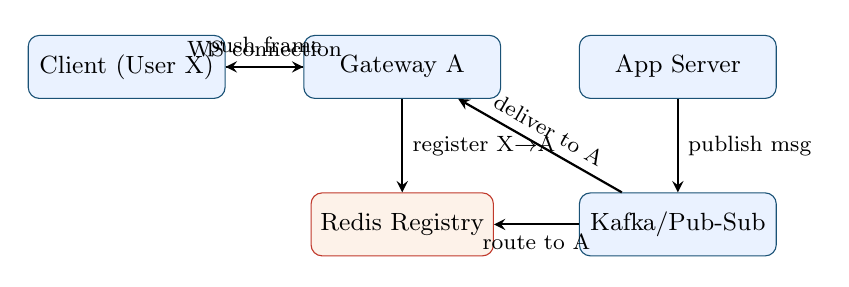
\begin{tikzpicture}[
  server/.style={rectangle, draw=highlight, fill=termbg, rounded corners, minimum width=2.5cm, minimum height=0.8cm, font=\small},
  store/.style={rectangle, draw=accent, fill=notebg, rounded corners, minimum width=2.2cm, minimum height=0.8cm, font=\small},
  arrow/.style={->, >=stealth, thick}
]
  \node[server] (client) at (0, 0) {Client (User X)};
  \node[server] (gwA) at (3.5, 0) {Gateway A};
  \node[store] (redis) at (3.5, -2) {Redis Registry};
  \node[server] (kafka) at (7, -2) {Kafka/Pub-Sub};
  \node[server] (app) at (7, 0) {App Server};

  \draw[arrow] (client) -- node[above, font=\footnotesize]{WS connection} (gwA);
  \draw[arrow] (gwA) -- node[right, font=\footnotesize]{register X$\to$A} (redis);
  \draw[arrow] (app) -- node[right, font=\footnotesize]{publish msg} (kafka);
  \draw[arrow] (kafka) -- node[below, font=\footnotesize]{route to A} (redis);
  \draw[arrow] (kafka) -- node[above, font=\footnotesize, sloped]{deliver to A} (gwA);
  \draw[arrow, dashed] (gwA) -- node[above, font=\footnotesize]{push frame} (client);
\end{tikzpicture}

\vspace{6pt}

% ── Section 6: Choosing the Right Mechanism ───────────────────────────────────
\section{Choosing the Right Mechanism: A Decision Framework}

Choosing between polling, long polling, SSE, and WebSockets is not a taste preference. It follows from the requirements.

\textbf{Does the client need to push data to the server through the same connection?} If yes, you need WebSockets. Chat, collaborative editing (Google Docs), live gaming, and trading platforms all have this requirement. SSE only flows server-to-client.

\textbf{Is the communication pattern strictly server-to-client?} If yes, prefer SSE over WebSockets. It's simpler to implement, simpler to proxy, and comes with automatic reconnection. Use it for notification feeds, live dashboards, progress indicators, and activity timelines.

\textbf{Do you need to support environments where WebSockets are blocked?} Corporate firewalls frequently block WebSocket upgrades. Libraries like Socket.IO handle this by falling back to long polling when WebSocket negotiation fails. This is a legitimate operational concern for enterprise products.

\textbf{Are you building internal service-to-service communication?} Then neither WebSockets nor SSE are the right tool. gRPC (which uses HTTP/2 streams with Protocol Buffer encoding) is the standard for service-to-service real-time communication. It provides bidirectional streaming, strong typing, and efficient binary encoding. The rule of thumb: WebSockets face client-side (browser, mobile app); gRPC faces service-side (microservice to microservice).

\begin{tabularx}{\linewidth}{lXXX}
\toprule
\textbf{Mechanism} & \textbf{Direction} & \textbf{Best For} & \textbf{Avoid When} \\
\midrule
Short polling & Client $\to$ Server only & Legacy systems & Always; use SSE or WS instead \\
Long polling & Server-initiated response & Simple push, broad compatibility & High connection concurrency \\
SSE & Server $\to$ Client & Feeds, dashboards, notifications & Client needs to push data \\
WebSocket & Bidirectional & Chat, gaming, collaboration, trading & One-way push only needed \\
gRPC streaming & Bidirectional & Service-to-service real-time & Browser clients (limited support) \\
\bottomrule
\end{tabularx}

% ── Section 7: Critical Numbers ───────────────────────────────────────────────
\section{Numbers Worth Memorizing}

The following numbers come up in system design interviews, either because interviewers quote them directly or because back-of-the-envelope calculations require them. Knowing them to one significant figure is sufficient.

\begin{tabularx}{\linewidth}{Xr}
\toprule
\textbf{Fact} & \textbf{Value} \\
\midrule
TCP 3-way handshake latency cost & $1.5 \times$ RTT \\
TLS 1.3 additional handshake cost (new session) & $+0.5$ RTT \\
TLS 1.3 0-RTT resumption cost & $0$ additional RTT \\
HTTP/1.1 keep-alive default timeout & 60--90 seconds \\
HTTP headers per request (typical) & 500--800 bytes \\
HTTP/2 HPACK compression savings & $\approx 85$\% \\
WebSocket frame header overhead & 2--14 bytes \\
HTTP/2 default max concurrent streams & 100 per connection \\
HTTP/3 adoption globally (late 2024) & 35\% of web traffic \\
HTTP/3 speed improvement at 15\% packet loss & 55\% faster than HTTP/2 \\
Concurrent TCP connections, tuned Linux server & 500K -- 1M \\
WebSocket connections per server (typical tuned) & 100K -- 1M \\
Memory per WebSocket connection & $\approx 50$ KB \\
1M WebSocket connections memory cost & $\approx 50$ GB RAM \\
APNs persistent connection port & 5223 \\
Browser parallel connections per domain (HTTP/1.1) & 6 \\
\bottomrule
\end{tabularx}

% ── Section 8: The Session_001 Error Explained ───────────────────────────────
\section{Why You Cannot Push to a Device IP Address}

Let's return to the session\_001 error and make it permanent.

When a phone connects to a cellular network, the carrier's infrastructure assigns it an IP address --- but it's a private IP address on the carrier's internal network. The carrier uses Network Address Translation (NAT) to share a pool of public IP addresses across millions of devices. From the internet's perspective, your phone is not visible at a stable, routable address. It exists behind layers of NAT that rewrite packet headers as traffic flows in and out.

The NAT rule is strict: traffic can flow \emph{out} from a device (the NAT gateway records the outgoing connection and knows to forward responses back), but nothing can initiate traffic \emph{in} to the device. There's no public IP to target. Even if there were, iOS and Android aggressively kill background processes and their network connections to preserve battery.

This is why Apple and Google built APNs and FCM respectively. The operating system itself --- not your app --- maintains a persistent TCP connection to Apple's servers (on port 5223) or Google's servers. This connection is privileged: the OS keeps it alive even when apps are suspended. Your notification server never talks to the device. It talks to APNs, which uses the existing OS-level connection to wake the app. The device is always the initiator. Always the client. Always.

\begin{insightbox}
\textbf{The mental model:} Your backend talks to a cloud (APNs/FCM), not to a device. The cloud talks to the OS, not to your app. The OS wakes your app. This is a two-hop relay, not a direct connection. Understanding these two hops is the difference between a correct notification architecture and a fundamentally broken one.
\end{insightbox}

% ── Curiosity Corner ──────────────────────────────────────────────────────────
\newpage
\section*{Curiosity Corner}
\addcontentsline{toc}{section}{Curiosity Corner}

\textit{These are the questions that likely occurred to you while reading. Take a moment to try answering each one before reading the explanation.}

\vspace{8pt}

\begin{curiobox}{If HTTP/3 is better, why hasn't it completely replaced HTTP/2?}
Three reasons. First, HTTP/3 requires UDP, and many enterprise firewalls block UDP entirely or severely throttle it for ports other than DNS (port 53). A site serving HTTP/3 to a user behind such a firewall falls back to HTTP/2 automatically, but it means the real deployment percentage is lower than adoption numbers suggest. Second, QUIC runs in user space, which means it consumes more CPU than TCP (which has decades of hardware and OS-level optimization). Cloudflare measured roughly 20\% higher CPU usage for QUIC vs TCP in 2021. This gap is narrowing, but it matters at scale. Third, the tooling ecosystem (packet analyzers, load balancers, proxies) is less mature for QUIC --- operational debugging is harder, which slows enterprise adoption.
\end{curiobox}

\vspace{6pt}

\begin{curiobox}{How does a load balancer handle WebSocket connections if they're stateful?}
Layer 4 (TCP) load balancers simply forward TCP connections. Since the WebSocket connection persists at the TCP level, the same connection stays on the same backend server for its entire lifetime. The load balancer doesn't need to do anything special --- it made a routing decision when the connection was established and then gets out of the way. Layer 7 (HTTP) load balancers must explicitly handle the WebSocket upgrade: they need to detect the \texttt{Upgrade: websocket} header and switch from request-response mode to pass-through TCP proxying mode. NGINX has supported this since version 1.3.13 (2012); HAProxy since version 1.4. The sticky session problem comes in when you're scaling WebSocket servers: if you have multiple gateway servers, the load balancer must keep sending the same user's reconnections to the same server (or your routing logic must handle transfers, which is complex). Most production systems use consistent hashing on the user ID to pin users to gateway servers.
\end{curiobox}

\vspace{6pt}

\begin{curiobox}{What's the actual difference between TCP's reliability and QUIC's reliability?}
Functionally, identical: both guarantee ordered, reliable delivery of application data. The implementation differs. TCP reliability lives in the OS kernel --- the kernel manages retransmission buffers, computes timeouts, and sends ACKs. QUIC reliability lives in user space --- the QUIC library (running as part of your application process) manages its own packet buffers, timeouts, and acknowledgments. This has a practical consequence: QUIC can be updated and improved without waiting for OS kernel releases. Google pushed multiple QUIC performance improvements in 2023 and 2024 through library updates, while TCP improvements require kernel upgrades that can take years to propagate. User-space networking also makes it easier to implement per-stream independent loss recovery, which is where QUIC's HOL-blocking advantage comes from.
\end{curiobox}

\vspace{6pt}

\begin{curiobox}{Why does the TCP TIME\_WAIT state exist and why do I see it in netstat?}
After a TCP connection closes, the initiating side enters TIME\_WAIT for 2 \texttimes MSL (Maximum Segment Lifetime --- typically 60 seconds, so TIME\_WAIT lasts 2 minutes). The reason: a delayed packet from the just-closed connection might still be in flight somewhere in the network. If a new connection used the same four-tuple (source IP, source port, dest IP, dest port) immediately, that delayed packet could be misinterpreted as belonging to the new connection. TIME\_WAIT prevents this. In production systems, you see thousands of TIME\_WAIT entries during periods of high connection churn (short-lived HTTP requests, microservice health checks). If TIME\_WAIT sockets are exhausting your port range, the solution is \texttt{SO\_REUSEADDR}, reducing MSL via \texttt{net.ipv4.tcp\_fin\_timeout}, or persistent connections to reduce connection churn.
\end{curiobox}

\vspace{6pt}

\begin{curiobox}{Is WebRTC the same as WebSocket?}
No. WebRTC (Web Real-Time Communication) is a completely separate technology stack designed specifically for peer-to-peer audio, video, and data communication between browsers. WebRTC uses UDP (via ICE/STUN/TURN for NAT traversal) and has its own protocols (SRTP for media, SCTP for data channels). WebSockets require a server in the middle; WebRTC establishes a direct connection between two browsers (using the server only for initial signaling). You'd use WebRTC for a Zoom-like video call where media needs to flow peer-to-peer with sub-second latency. You'd use WebSockets for a Slack-like chat where messages route through your backend (which needs to store them, moderate them, sync them across devices). Some collaborative applications combine both: WebSockets for document state sync, WebRTC for live video during a collaborative session.
\end{curiobox}

\vspace{6pt}

\begin{curiobox}{What is gRPC and when does it beat WebSockets?}
gRPC is a remote procedure call framework built on HTTP/2, using Protocol Buffers as its serialization format. It supports four call patterns: unary (one request, one response --- identical to HTTP), server streaming (one request, stream of responses), client streaming (stream of requests, one response), and bidirectional streaming (both sides stream simultaneously). gRPC beats WebSockets for service-to-service communication because it provides a typed interface definition (proto files), automatic code generation in many languages, HTTP/2 multiplexing, and binary serialization. It does not beat WebSockets for browser clients --- browser gRPC support requires a translation layer called gRPC-Web, which loses some features. In practice: use gRPC between your backend services; use WebSockets (or SSE) between your servers and browser/mobile clients.
\end{curiobox}

% ── Self-Quiz ─────────────────────────────────────────────────────────────────
\newpage
\section*{Self-Quiz}
\addcontentsline{toc}{section}{Self-Quiz}

\textit{These are the actual probes an interviewer uses. Answer them before reading the model answers below. Cover the answers page while you work through these.}

\vspace{8pt}

\begin{quizbox}
\textbf{Q1 [Foundation]:} An engineer on your team suggests your real-time notification service can push notifications by opening a TCP connection to the user's device IP and sending a packet. Explain precisely why this won't work and describe the correct architecture.

\vspace{10pt}

\textbf{Q2 [Design]:} You're designing WhatsApp. You have 50M concurrent users online. Your architecture has 200 WebSocket gateway servers. User A is connected to gateway server 43. User B sends a message to User A. Walk through the full message delivery path from User B's phone to User A's phone.

\vspace{10pt}

\textbf{Q3 [Tradeoffs]:} Your product manager wants to add a live notification count badge to your web dashboard that updates in real-time when new notifications arrive. A junior engineer suggests WebSockets. You suggest SSE instead. Defend your choice. Under what conditions would the junior engineer be right?

\vspace{10pt}

\textbf{Q4 [Performance]:} Your API serves global users and you're seeing high tail latency (p99 = 3 seconds) on your HTTP/2 endpoints for users in Southeast Asia and India. Your infrastructure team suggests HTTP/3. Is this the right diagnosis? What else would you check first?

\vspace{10pt}

\textbf{Q5 [Scaling]:} You're asked to design the WebSocket gateway layer for a chat system that must support 10M concurrent connections. Walk through the capacity planning: how many servers do you need, how are connections distributed, and how does a message reach the correct server?
\end{quizbox}

\newpage
\begin{answerbox}
\textbf{A1:} Consumer devices operate behind NAT --- the carrier or ISP assigns them private IPs and uses NAT to share public IPs. No stable, routable public IP exists for the device, so no external server can initiate a TCP connection to it. Even if it could, mobile OSes kill background processes and their network connections. The correct architecture: (1) The OS maintains a persistent TCP connection to APNs (port 5223) or FCM. (2) Your backend sends the notification payload to APNs/FCM via their server-side API. (3) APNs/FCM uses the existing OS-level connection to deliver the notification and wake the app. The device is always the initiator. Your backend never communicates with the device directly.

\vspace{8pt}

\textbf{A2:} User B's phone sends the message over its WebSocket to whichever gateway server User B is connected to (say, server 81). Gateway 81 persists the message to your message store (e.g., Cassandra or PostgreSQL). It then looks up User A's connection entry in the connection registry (Redis hash: \texttt{user\_a $\to$ gateway\_43}). Gateway 81 publishes the message to a Pub/Sub channel for User A (e.g., Redis Pub/Sub channel \texttt{user:A:inbox}, or a Kafka partition keyed by User A's ID). Gateway 43, which holds User A's WebSocket and is subscribed to that channel, receives the published message and pushes it over User A's WebSocket frame. If User A is offline (no entry in registry), the message stays in the message store and is delivered when they reconnect.

\vspace{8pt}

\textbf{A3:} SSE is correct for a notification badge counter because the data flows in one direction: server to client. The client never needs to push notification data \emph{back} through the same connection --- interactions (clicking, dismissing) go through standard HTTP POST requests. SSE is simpler (no upgrade handshake), proxies correctly without special configuration, reconnects automatically, and doesn't consume the bidirectional channel capacity that WebSockets provide. The junior engineer would be right if the dashboard also needed to \emph{send} real-time data to the server through the same connection --- for example, if users could collaborate on shared documents visible in the dashboard and edits needed to propagate with sub-second latency.

\vspace{8pt}

\textbf{A4:} HTTP/3 is a reasonable hypothesis but not the first thing to check. First: verify whether the high p99 is concentrated in specific regions or across all users (if only Southeast Asia, the issue may be routing, not protocol). Second: check whether your CDN has a presence in the region --- if users are hitting your origin directly from 200ms away, that's the problem; HTTP/3 saves 1.5 RTT on new connections but doesn't help if bandwidth is the bottleneck. Third: profile what happens in those 3 seconds --- is it DNS resolution, TCP handshake, TLS negotiation, server processing time, or response transfer? HTTP/3 helps with handshake cost and packet-loss recovery, but not with server processing time. If after investigation the issue is repeated TLS renegotiation under poor connectivity, then yes, HTTP/3's 0-RTT resumption and connection migration are the right solution.

\vspace{8pt}

\textbf{A5:} At 50KB per connection, 10M connections require 500GB of total connection memory. Assuming 64GB RAM servers (typical cloud instance), you need at minimum $\lceil 500/64 \rceil = 8$ servers for memory alone, but you'd over-provision to 20--30 for fault tolerance and headroom. Distribute connections using consistent hashing on user ID: this ensures that when a server goes down and connections are redistributed, only the connections from that server move (not all 10M). The connection registry (user ID $\to$ server ID) lives in Redis, which can handle millions of keys with sub-millisecond lookups. For message routing between servers, use a Pub/Sub layer (Kafka for durability, Redis Pub/Sub for lower latency). Each gateway server subscribes to the channels for users it currently hosts. A consistent-hash ring manages the mapping, and the registry is the source of truth.
\end{answerbox}

% ── What's Next ───────────────────────────────────────────────────────────────
\vspace{16pt}
\begin{insightbox}
\textbf{Next: L1-02 --- Push Delivery: APNs \& FCM}

You now understand why devices cannot receive inbound connections and why persistent OS-level connections are the solution. L1-02 goes inside APNs and FCM: device token registration and rotation, the APNS binary protocol, quality of service tiers (Priority 5 vs Priority 10), store-and-forward behavior, silent push vs display push, expiration handling, and how your backend authenticates with Apple's and Google's servers. This is the lesson that directly repairs the session\_001 critical gap.

\textbf{After L1-02:} L1-08 (Message Queues) gives you the async pipeline that connects your application to your APNs/FCM delivery layer at scale. Together, L1-01 + L1-02 + L1-08 form the complete foundation for designing any notification system at the senior interview level.
\end{insightbox}

\vspace{12pt}
{\color{highlight!50}\rule{\linewidth}{0.6pt}}
\begin{center}
\small\color{primary!60}
\textit{L1-01 complete} \quad\textbullet\quad
\textit{Mark \texttt{curriculum/progress.md} as done} \quad\textbullet\quad
\textit{When ready, start L1-02}
\end{center}

\end{document}
